\documentclass[a4paper, 11pt]{article}

%\usepackage[center]{titlesec}

\usepackage{amsfonts, amssymb, amsmath, amsthm, amsxtra}

\usepackage{foekfont}

\usepackage{MnSymbol}

\usepackage{pdfrender, xcolor}
%\pdfrender{StrokeColor=black,LineWidth=.4pt,TextRenderingMode=2}

%\usepackage{minitoc}
%\setcounter{section}{-1}
%\setcounter{tocdepth}{}
%\setcounter{minitocdepth}{}
%\setcounter{secnumdepth}{}

\usepackage{graphicx}

\usepackage[english]{babel}
\usepackage[utf8]{inputenc}
%\usepackage{mathpazo}
%\usepackage{eucal}
\usepackage{eufrak}
\usepackage{bbm}
\usepackage{bm}
\usepackage{csquotes}
\usepackage[nottoc]{tocbibind}
\usepackage{appendix}
\usepackage{float}
\usepackage[T1]{fontenc}
\usepackage[
    left = \flqq{},% 
    right = \frqq{},% 
    leftsub = \flq{},% 
    rightsub = \frq{} %
]{dirtytalk}

\usepackage{imakeidx}
\makeindex

%\usepackage[dvipsnames]{xcolor}
\usepackage{hyperref}
    \hypersetup{
        colorlinks=true,
        linkcolor=teal,
        filecolor=pink,      
        urlcolor=teal,
        citecolor=magenta
    }
\usepackage{comment}

% You would set the PDF title, author, etc. with package options or
% \hypersetup.

\usepackage[backend=biber, style=alphabetic, sorting=nty]{biblatex}
    \addbibresource{bibliography.bib}
\renewbibmacro{in:}{}

\raggedbottom

\usepackage{mathrsfs}
\usepackage{mathtools} 
\mathtoolsset{showonlyrefs} 
%\usepackage{amsthm}
\renewcommand\qedsymbol{$\blacksquare$}

\usepackage{tikz-cd}
\tikzcdset{scale cd/.style={every label/.append style={scale=#1},
    cells={nodes={scale=#1}}}}
\usepackage{tikz}
\usepackage{setspace}
\usepackage[version=3]{mhchem}
\parskip=0.1in
\usepackage[margin=25mm]{geometry}

\usepackage{listings, lstautogobble}
\lstset{
	language=matlab,
	basicstyle=\scriptsize\ttfamily,
	commentstyle=\ttfamily\itshape\color{gray},
	stringstyle=\ttfamily,
	showstringspaces=false,
	breaklines=true,
	frameround=ffff,
	frame=single,
	rulecolor=\color{black},
	autogobble=true
}

\usepackage{todonotes,tocloft,xpatch,hyperref}

% This is based on classicthesis chapter definition
\let\oldsec=\section
\renewcommand*{\section}{\secdef{\Sec}{\SecS}}
\newcommand\SecS[1]{\oldsec*{#1}}%
\newcommand\Sec[2][]{\oldsec[\texorpdfstring{#1}{#1}]{#2}}%

\newcounter{istodo}[section]

% http://tex.stackexchange.com/a/61267/11984
\makeatletter
%\xapptocmd{\Sec}{\addtocontents{tdo}{\protect\todoline{\thesection}{#1}{}}}{}{}
\newcommand{\todoline}[1]{\@ifnextchar\Endoftdo{}{\@todoline{#1}}}
\newcommand{\@todoline}[3]{%
	\@ifnextchar\todoline{}
	{\contentsline{section}{\numberline{#1}#2}{#3}{}{}}%
}
\let\l@todo\l@subsection
\newcommand{\Endoftdo}{}

\AtEndDocument{\addtocontents{tdo}{\string\Endoftdo}}
\makeatother

\usepackage{lipsum}

%   Reduce the margin of the summary:
\def\changemargin#1#2{\list{}{\rightmargin#2\leftmargin#1}\item[]}
\let\endchangemargin=\endlist 

%   Generate the environment for the abstract:
%\newcommand\summaryname{Abstract}
%\newenvironment{abstract}%
    %{\small\begin{center}%
    %\bfseries{\summaryname} \end{center}}

\newtheorem{theorem}{Theorem}[section]
    \numberwithin{theorem}{subsection}
\newtheorem{proposition}{Proposition}[section]
    \numberwithin{proposition}{subsection}
\newtheorem{lemma}{Lemma}[section]
    \numberwithin{lemma}{subsection}
\newtheorem{claim}{Claim}[section]
    \numberwithin{claim}{subsection}
\newtheorem{question}{Question}[section]
    \numberwithin{question}{subsection}

\theoremstyle{definition}
    \newtheorem{definition}{Definition}[section]
        \numberwithin{definition}{subsection}

\theoremstyle{remark}
    \newtheorem{remark}{Remark}[section]
        \numberwithin{remark}{subsection}
    \newtheorem{example}{Example}[section]
        \numberwithin{example}{subsection}    
    \newtheorem{convention}{Convention}[section]
        \numberwithin{convention}{subsection}
    \newtheorem{corollary}{Corollary}[section]
        \numberwithin{corollary}{subsection}

\numberwithin{equation}{section}

\setcounter{section}{-1}

\renewcommand{\cong}{\simeq}
\newcommand{\ladjoint}{\dashv}
\newcommand{\radjoint}{\vdash}
\newcommand{\<}{\langle}
\renewcommand{\>}{\rangle}
\newcommand{\ndiv}{\hspace{-2pt}\not|\hspace{5pt}}
\newcommand{\cond}{\blacktriangle}
\newcommand{\decond}{\triangle}
\newcommand{\solid}{\blacksquare}
\newcommand{\ot}{\leftarrow}
\renewcommand{\-}{\text{-}}
\renewcommand{\mapsto}{\leadsto}
\renewcommand{\leq}{\leqslant}
\renewcommand{\geq}{\geqslant}
\renewcommand{\setminus}{\smallsetminus}
\makeatletter
\DeclareRobustCommand{\cev}[1]{%
  {\mathpalette\do@cev{#1}}%
}
\newcommand{\do@cev}[2]{%
  \vbox{\offinterlineskip
    \sbox\z@{$\m@th#1 x$}%
    \ialign{##\cr
      \hidewidth\reflectbox{$\m@th#1\vec{}\mkern4mu$}\hidewidth\cr
      \noalign{\kern-\ht\z@}
      $\m@th#1#2$\cr
    }%
  }%
}
\makeatother

\newcommand{\N}{\mathbb{N}}
\newcommand{\Z}{\mathbb{Z}}
\newcommand{\Q}{\mathbb{Q}}
\newcommand{\R}{\mathbb{R}}
\newcommand{\bbC}{\mathbb{C}}
\NewDocumentCommand{\x}{e{_^}}{%
  \mathbin{\mathop{\times}\displaylimits
    \IfValueT{#1}{_{#1}}
    \IfValueT{#2}{^{#2}}
  }%
}
\NewDocumentCommand{\pushout}{e{_^}}{%
  \mathbin{\mathop{\sqcup}\displaylimits
    \IfValueT{#1}{_{#1}}
    \IfValueT{#2}{^{#2}}
  }%
}
\newcommand{\supp}{\operatorname{supp}}
\newcommand{\im}{\operatorname{im}}
\newcommand{\coker}{\operatorname{coker}}
\newcommand{\id}{\mathrm{id}}
\newcommand{\chara}{\operatorname{char}}
\newcommand{\trdeg}{\operatorname{trdeg}}
\newcommand{\rank}{\operatorname{rank}}
\newcommand{\trace}{\operatorname{tr}}
\newcommand{\length}{\operatorname{length}}
\newcommand{\height}{\operatorname{ht}}
\renewcommand{\span}{\operatorname{span}}
\newcommand{\e}{\epsilon}
\newcommand{\p}{\mathfrak{p}}
\newcommand{\q}{\mathfrak{q}}
\newcommand{\m}{\mathfrak{m}}
\newcommand{\n}{\mathfrak{n}}
\newcommand{\calF}{\mathcal{F}}
\newcommand{\calG}{\mathcal{G}}
\newcommand{\calO}{\mathcal{O}}
\newcommand{\F}{\mathbb{F}}
\DeclareMathOperator{\lcm}{lcm}
\newcommand{\gr}{\operatorname{gr}}
\newcommand{\vol}{\mathrm{vol}}
\newcommand{\ord}{\operatorname{ord}}
\newcommand{\projdim}{\operatorname{proj.dim}}
\newcommand{\injdim}{\operatorname{inj.dim}}
\newcommand{\flatdim}{\operatorname{flat.dim}}
\newcommand{\globdim}{\operatorname{glob.dim}}
\renewcommand{\Re}{\operatorname{Re}}
\renewcommand{\Im}{\operatorname{Im}}
\newcommand{\sgn}{\operatorname{sgn}}
\newcommand{\coad}{\operatorname{coad}}

\newcommand{\Ad}{\mathrm{Ad}}
\newcommand{\GL}{\mathrm{GL}}
\newcommand{\SL}{\mathrm{SL}}
\newcommand{\PGL}{\mathrm{PGL}}
\newcommand{\PSL}{\mathrm{PSL}}
\newcommand{\Sp}{\mathrm{Sp}}
\newcommand{\GSp}{\mathrm{GSp}}
\newcommand{\GSpin}{\mathrm{GSpin}}
\newcommand{\rmO}{\mathrm{O}}
\newcommand{\SO}{\mathrm{SO}}
\newcommand{\SU}{\mathrm{SU}}
\newcommand{\rmU}{\mathrm{U}}
\newcommand{\rmu}{\mathrm{u}}
\newcommand{\rmV}{\mathrm{V}}
\newcommand{\gl}{\mathfrak{gl}}
\renewcommand{\sl}{\mathfrak{sl}}
\newcommand{\diag}{\mathfrak{diag}}
\newcommand{\pgl}{\mathfrak{pgl}}
\newcommand{\psl}{\mathfrak{psl}}
\newcommand{\fraksp}{\mathfrak{sp}}
\newcommand{\gsp}{\mathfrak{gsp}}
\newcommand{\gspin}{\mathfrak{gspin}}
\newcommand{\frako}{\mathfrak{o}}
\newcommand{\so}{\mathfrak{so}}
\newcommand{\su}{\mathfrak{su}}
%\newcommand{\fraku}{\mathfrak{u}}
\newcommand{\Spec}{\operatorname{Spec}}
\newcommand{\Spf}{\operatorname{Spf}}
\newcommand{\Spm}{\operatorname{Spm}}
\newcommand{\Spv}{\operatorname{Spv}}
\newcommand{\Spa}{\operatorname{Spa}}
\newcommand{\Spd}{\operatorname{Spd}}
\newcommand{\Proj}{\operatorname{Proj}}
\newcommand{\Gr}{\mathrm{Gr}}
\newcommand{\Hecke}{\mathrm{Hecke}}
\newcommand{\Sht}{\mathrm{Sht}}
\newcommand{\Quot}{\mathrm{Quot}}
\newcommand{\Hilb}{\mathrm{Hilb}}
\newcommand{\Pic}{\mathrm{Pic}}
\newcommand{\Div}{\mathrm{Div}}
\newcommand{\Jac}{\mathrm{Jac}}
\newcommand{\Alb}{\mathrm{Alb}} %albanese variety
\newcommand{\Bun}{\mathrm{Bun}}
\newcommand{\loopspace}{\mathbf{\Omega}}
\newcommand{\suspension}{\mathbf{\Sigma}}
\newcommand{\tangent}{\mathrm{T}} %tangent space
\newcommand{\Eig}{\mathrm{Eig}}
\newcommand{\Cox}{\mathrm{Cox}} %coxeter functors
\newcommand{\rmK}{\mathrm{K}} %Killing form
\newcommand{\km}{\mathfrak{km}} %kac-moody algebras
\newcommand{\Dyn}{\mathrm{Dyn}} %associated Dynkin quivers
\newcommand{\Car}{\mathrm{Car}} %cartan matrices of finite quivers

\newcommand{\Ring}{\mathrm{Ring}}
\newcommand{\Cring}{\mathrm{CRing}}
\newcommand{\Alg}{\mathrm{Alg}}
\newcommand{\Leib}{\mathrm{Leib}} %leibniz algebras
\newcommand{\Fld}{\mathrm{Fld}}
\newcommand{\Sets}{\mathrm{Sets}}
\newcommand{\Equiv}{\mathrm{Equiv}} %equivalence relations
\newcommand{\Cat}{\mathrm{Cat}}
\newcommand{\Grp}{\mathrm{Grp}}
\newcommand{\Ab}{\mathrm{Ab}}
\newcommand{\Sch}{\mathrm{Sch}}
\newcommand{\Coh}{\mathrm{Coh}}
\newcommand{\QCoh}{\mathrm{QCoh}}
\newcommand{\Perf}{\mathrm{Perf}} %perfect complexes
\newcommand{\Sing}{\mathrm{Sing}} %singularity categories
\newcommand{\Desc}{\mathrm{Desc}}
\newcommand{\Sh}{\mathrm{Sh}}
\newcommand{\Psh}{\mathrm{PSh}}
\newcommand{\Fib}{\mathrm{Fib}}
\renewcommand{\mod}{\-\mathrm{mod}}
\newcommand{\comod}{\-\mathrm{comod}}
\newcommand{\bimod}{\-\mathrm{bimod}}
\newcommand{\Vect}{\mathrm{Vect}}
\newcommand{\Rep}{\mathrm{Rep}}
\newcommand{\Grpd}{\mathrm{Grpd}}
\newcommand{\Arr}{\mathrm{Arr}}
\newcommand{\Esp}{\mathrm{Esp}}
\newcommand{\Ob}{\mathrm{Ob}}
\newcommand{\Mor}{\mathrm{Mor}}
\newcommand{\Mfd}{\mathrm{Mfd}}
\newcommand{\Riem}{\mathrm{Riem}}
\newcommand{\RS}{\mathrm{RS}}
\newcommand{\LRS}{\mathrm{LRS}}
\newcommand{\TRS}{\mathrm{TRS}}
\newcommand{\TLRS}{\mathrm{TLRS}}
\newcommand{\LVRS}{\mathrm{LVRS}}
\newcommand{\LBRS}{\mathrm{LBRS}}
\newcommand{\Spc}{\mathrm{Spc}}
\newcommand{\Top}{\mathrm{Top}}
\newcommand{\Topos}{\mathrm{Topos}}
\newcommand{\Nil}{\mathfrak{nil}}
\newcommand{\J}{\mathfrak{J}}
\newcommand{\Stk}{\mathrm{Stk}}
\newcommand{\Pre}{\mathrm{Pre}}
\newcommand{\simp}{\mathbf{\Delta}}
\newcommand{\Res}{\mathrm{Res}}
\newcommand{\Ind}{\mathrm{Ind}}
\newcommand{\Pro}{\mathrm{Pro}}
\newcommand{\Mon}{\mathrm{Mon}}
\newcommand{\Comm}{\mathrm{Comm}}
\newcommand{\Fin}{\mathrm{Fin}}
\newcommand{\Assoc}{\mathrm{Assoc}}
\newcommand{\Semi}{\mathrm{Semi}}
\newcommand{\Co}{\mathrm{Co}}
\newcommand{\Loc}{\mathrm{Loc}}
\newcommand{\Ringed}{\mathrm{Ringed}}
\newcommand{\Haus}{\mathrm{Haus}} %hausdorff spaces
\newcommand{\Comp}{\mathrm{Comp}} %compact hausdorff spaces
\newcommand{\Stone}{\mathrm{Stone}} %stone spaces
\newcommand{\Extr}{\mathrm{Extr}} %extremely disconnected spaces
\newcommand{\Ouv}{\mathrm{Ouv}}
\newcommand{\Str}{\mathrm{Str}}
\newcommand{\Func}{\mathrm{Func}}
\newcommand{\Crys}{\mathrm{Crys}}
\newcommand{\LocSys}{\mathrm{LocSys}}
\newcommand{\Sieves}{\mathrm{Sieves}}
\newcommand{\pt}{\mathrm{pt}}
\newcommand{\Graphs}{\mathrm{Graphs}}
\newcommand{\Lie}{\mathrm{Lie}}
\newcommand{\Env}{\mathrm{Env}}
\newcommand{\Ho}{\mathrm{Ho}}
\newcommand{\rmD}{\mathrm{D}}
\newcommand{\Cov}{\mathrm{Cov}}
\newcommand{\Frames}{\mathrm{Frames}}
\newcommand{\Locales}{\mathrm{Locales}}
\newcommand{\Span}{\mathrm{Span}}
\newcommand{\Corr}{\mathrm{Corr}}
\newcommand{\Monad}{\mathrm{Monad}}
\newcommand{\Var}{\mathrm{Var}}
\newcommand{\sfN}{\mathrm{N}} %nerve
\newcommand{\Diam}{\mathrm{Diam}} %diamonds
\newcommand{\co}{\mathrm{co}}
\newcommand{\ev}{\mathrm{ev}}
\newcommand{\bi}{\mathrm{bi}}
\newcommand{\Nat}{\mathrm{Nat}}
\newcommand{\Hopf}{\mathrm{Hopf}}
\newcommand{\Dmod}{\mathrm{D}\mod}
\newcommand{\Perv}{\mathrm{Perv}}
\newcommand{\Sph}{\mathrm{Sph}}
\newcommand{\Moduli}{\mathrm{Moduli}}
\newcommand{\Pseudo}{\mathrm{Pseudo}}
\newcommand{\Lax}{\mathrm{Lax}}
\newcommand{\Strict}{\mathrm{Strict}}
\newcommand{\Opd}{\mathrm{Opd}} %operads
\newcommand{\Shv}{\mathrm{Shv}}
\newcommand{\Char}{\mathrm{Char}} %CharShv = character sheaves
\newcommand{\Huber}{\mathrm{Huber}}
\newcommand{\Tate}{\mathrm{Tate}}
\newcommand{\Affd}{\mathrm{Affd}} %affinoid algebras
\newcommand{\Adic}{\mathrm{Adic}} %adic spaces
\newcommand{\Rig}{\mathrm{Rig}}
\newcommand{\An}{\mathrm{An}}
\newcommand{\Perfd}{\mathrm{Perfd}} %perfectoid spaces
\newcommand{\Sub}{\mathrm{Sub}} %subobjects
\newcommand{\Ideals}{\mathrm{Ideals}}
\newcommand{\Isoc}{\mathrm{Isoc}} %isocrystals
\newcommand{\Ban}{\-\mathrm{Ban}} %Banach spaces
\newcommand{\Fre}{\-\mathrm{Fr\acute{e}}} %Frechet spaces
\newcommand{\Ch}{\mathrm{Ch}} %chain complexes
\newcommand{\Pure}{\mathrm{Pure}}
\newcommand{\Mixed}{\mathrm{Mixed}}
\newcommand{\Hodge}{\mathrm{Hodge}} %Hodge structures
\newcommand{\Mot}{\mathrm{Mot}} %motives
\newcommand{\KL}{\mathrm{KL}} %category of Kazhdan-Lusztig modules
\newcommand{\Pres}{\mathrm{Pres}} %presentable categories
\newcommand{\Noohi}{\mathrm{Noohi}} %category of Noohi groups
\newcommand{\Inf}{\mathrm{Inf}}
\newcommand{\LPar}{\mathrm{LPar}} %Langlands parameters
\newcommand{\ORig}{\mathrm{ORig}} %overconvergent sites
\newcommand{\Quiv}{\mathrm{Quiv}} %quivers
\newcommand{\Def}{\mathrm{Def}} %deformation functors
\newcommand{\Root}{\mathrm{Root}}
\newcommand{\gRep}{\mathrm{gRep}}
\newcommand{\Higgs}{\mathrm{Higgs}}
\newcommand{\BGG}{\mathrm{BGG}}

\newcommand{\Aut}{\mathrm{Aut}}
\newcommand{\Inn}{\mathrm{Inn}}
\newcommand{\Out}{\mathrm{Out}}
\newcommand{\der}{\mathfrak{der}} %derivations on Lie algebras
\newcommand{\frakend}{\mathfrak{end}}
\newcommand{\aut}{\mathfrak{aut}}
\newcommand{\inn}{\mathfrak{inn}} %inner derivations
\newcommand{\out}{\mathfrak{out}} %outer derivations
\newcommand{\Stab}{\mathrm{Stab}}
\newcommand{\Cent}{\mathrm{Cent}}
\newcommand{\Norm}{\mathrm{Norm}}
\newcommand{\stab}{\mathfrak{stab}}
\newcommand{\cent}{\mathfrak{cent}}
\newcommand{\norm}{\mathfrak{norm}}
\newcommand{\Rad}{\operatorname{Rad}}
\newcommand{\Transporter}{\mathrm{Transp}} %transporter between two subsets of a group
\newcommand{\Conj}{\mathrm{Conj}}
\newcommand{\Diag}{\mathrm{Diag}}
\newcommand{\Gal}{\mathrm{Gal}}
\newcommand{\bfG}{\mathbf{G}} %absolute Galois group
\newcommand{\Frac}{\mathrm{Frac}}
\newcommand{\Ann}{\mathrm{Ann}}
\newcommand{\Val}{\mathrm{Val}}
\newcommand{\Chow}{\mathrm{Chow}}
\newcommand{\Sym}{\mathrm{Sym}}
\newcommand{\End}{\mathrm{End}}
\newcommand{\Mat}{\mathrm{Mat}}
\newcommand{\Diff}{\mathrm{Diff}}
\newcommand{\Autom}{\mathrm{Autom}}
\newcommand{\Artin}{\mathrm{Artin}} %artin maps
\newcommand{\sk}{\mathrm{sk}} %skeleton of a category
\newcommand{\eqv}{\mathrm{eqv}} %functor that maps groups $G$ to $G$-sets
\newcommand{\Inert}{\mathrm{Inert}}
\newcommand{\Fil}{\mathrm{Fil}}
\newcommand{\Prim}{\mathfrak{Prim}}
\newcommand{\Nerve}{\mathrm{N}}
\newcommand{\Hol}{\mathrm{Hol}} %holomorphic functions %holonomy groups
\newcommand{\Bi}{\mathrm{Bi}} %Bi for biholomorphic functions
\newcommand{\chev}{\mathfrak{chev}} %chevalley relations
\newcommand{\bfLie}{\mathbf{Lie}} %non-reduced lie algebra associated to generalised cartan matrices
\newcommand{\frakLie}{\mathfrak{Lie}} %reduced lie algebra associated to generalised cartan matrices
\newcommand{\frakChev}{\mathfrak{Chev}} 
\newcommand{\Rees}{\operatorname{Rees}}
\newcommand{\Dr}{\mathrm{Dr}} %Drinfeld's quantum double 

\renewcommand{\projlim}{\varprojlim}
\newcommand{\indlim}{\varinjlim}
\newcommand{\colim}{\operatorname{colim}}
\renewcommand{\lim}{\operatorname{lim}}
\newcommand{\toto}{\rightrightarrows}
%\newcommand{\tensor}{\otimes}
\NewDocumentCommand{\tensor}{e{_^}}{%
  \mathbin{\mathop{\otimes}\displaylimits
    \IfValueT{#1}{_{#1}}
    \IfValueT{#2}{^{#2}}
  }%
}
\NewDocumentCommand{\singtensor}{e{_^}}{%
  \mathbin{\mathop{\odot}\displaylimits
    \IfValueT{#1}{_{#1}}
    \IfValueT{#2}{^{#2}}
  }%
}
\NewDocumentCommand{\hattensor}{e{_^}}{%
  \mathbin{\mathop{\hat{\otimes}}\displaylimits
    \IfValueT{#1}{_{#1}}
    \IfValueT{#2}{^{#2}}
  }%
}
\NewDocumentCommand{\semidirect}{e{_^}}{%
  \mathbin{\mathop{\rtimes}\displaylimits
    \IfValueT{#1}{_{#1}}
    \IfValueT{#2}{^{#2}}
  }%
}
\newcommand{\eq}{\operatorname{eq}}
\newcommand{\coeq}{\operatorname{coeq}}
\newcommand{\Hom}{\mathrm{Hom}}
\newcommand{\Maps}{\mathrm{Maps}}
\newcommand{\Tor}{\mathrm{Tor}}
\newcommand{\Ext}{\mathrm{Ext}}
\newcommand{\Isom}{\mathrm{Isom}}
\newcommand{\stalk}{\mathrm{stalk}}
\newcommand{\RKE}{\operatorname{RKE}}
\newcommand{\LKE}{\operatorname{LKE}}
\newcommand{\oblv}{\mathrm{oblv}}
\newcommand{\const}{\mathrm{const}}
\newcommand{\free}{\mathrm{free}}
\newcommand{\adrep}{\mathrm{ad}} %adjoint representation
\newcommand{\NL}{\mathbb{NL}} %naive cotangent complex
\newcommand{\pr}{\operatorname{pr}}
\newcommand{\Der}{\mathrm{Der}}
\newcommand{\Frob}{\mathrm{Fr}} %Frobenius
\newcommand{\frob}{\mathrm{f}} %trace of Frobenius
\newcommand{\bfpt}{\mathbf{pt}}
\newcommand{\bfloc}{\mathbf{loc}}
\DeclareMathAlphabet{\mymathbb}{U}{BOONDOX-ds}{m}{n}
\newcommand{\0}{\mymathbb{0}}
\newcommand{\1}{\mathbbm{1}}
\newcommand{\2}{\mathbbm{2}}
\newcommand{\Jet}{\mathrm{Jet}}
\newcommand{\Split}{\mathrm{Split}}
\newcommand{\Sq}{\mathrm{Sq}}
\newcommand{\Zero}{\mathrm{Z}}
\newcommand{\SqZ}{\Sq\Zero}
\newcommand{\lie}{\mathfrak{lie}}
\newcommand{\y}{\mathrm{y}} %yoneda
\newcommand{\Sm}{\mathrm{Sm}}
\newcommand{\AJ}{\phi} %abel-jacobi map
\newcommand{\act}{\mathrm{act}}
\newcommand{\ram}{\mathrm{ram}} %ramification index
\newcommand{\inv}{\mathrm{inv}}
\newcommand{\Spr}{\mathrm{Spr}} %the Springer map/sheaf
\newcommand{\Refl}{\mathrm{Refl}} %reflection functor]
\newcommand{\HH}{\mathrm{HH}} %Hochschild (co)homology
\newcommand{\Poinc}{\mathrm{Poinc}}
\newcommand{\Simpson}{\mathrm{Simpson}}

\newcommand{\bbU}{\mathbb{U}}
\newcommand{\V}{\mathbb{V}}
\newcommand{\calU}{\mathcal{U}}
\newcommand{\calW}{\mathcal{W}}
\newcommand{\rmI}{\mathrm{I}} %augmentation ideal
\newcommand{\bfV}{\mathbf{V}}
\newcommand{\C}{\mathcal{C}}
\newcommand{\D}{\mathcal{D}}
\newcommand{\T}{\mathscr{T}} %Tate modules
\newcommand{\calM}{\mathcal{M}}
\newcommand{\calN}{\mathcal{N}}
\newcommand{\calP}{\mathcal{P}}
\newcommand{\calQ}{\mathcal{Q}}
\newcommand{\A}{\mathbb{A}}
\renewcommand{\P}{\mathbb{P}}
\newcommand{\calL}{\mathcal{L}}
\newcommand{\E}{\mathcal{E}}
\renewcommand{\H}{\mathbf{H}}
\newcommand{\scrS}{\mathscr{S}}
\newcommand{\calX}{\mathcal{X}}
\newcommand{\calY}{\mathcal{Y}}
\newcommand{\calZ}{\mathcal{Z}}
\newcommand{\calS}{\mathcal{S}}
\newcommand{\calR}{\mathcal{R}}
\newcommand{\scrX}{\mathscr{X}}
\newcommand{\scrY}{\mathscr{Y}}
\newcommand{\scrZ}{\mathscr{Z}}
\newcommand{\calA}{\mathcal{A}}
\newcommand{\calB}{\mathcal{B}}
\renewcommand{\S}{\mathcal{S}}
\newcommand{\B}{\mathbb{B}}
\newcommand{\bbD}{\mathbb{D}}
\newcommand{\G}{\mathbb{G}}
\newcommand{\horn}{\mathbf{\Lambda}}
\renewcommand{\L}{\mathbb{L}}
\renewcommand{\a}{\mathfrak{a}}
\renewcommand{\b}{\mathfrak{b}}
\renewcommand{\c}{\mathfrak{c}}
\renewcommand{\t}{\mathfrak{t}}
\renewcommand{\r}{\mathfrak{r}}
\newcommand{\fraku}{\mathfrak{u}}
\newcommand{\bbX}{\mathbb{X}}
\newcommand{\frakw}{\mathfrak{w}}
\newcommand{\frakG}{\mathfrak{G}}
\newcommand{\frakH}{\mathfrak{H}}
\newcommand{\frakE}{\mathfrak{E}}
\newcommand{\frakF}{\mathfrak{F}}
\newcommand{\g}{\mathfrak{g}}
\newcommand{\h}{\mathfrak{h}}
\renewcommand{\k}{\mathfrak{k}}
\newcommand{\z}{\mathfrak{z}}
\newcommand{\fraki}{\mathfrak{i}}
\newcommand{\frakj}{\mathfrak{j}}
\newcommand{\del}{\partial}
\newcommand{\bbE}{\mathbb{E}}
\newcommand{\scrO}{\mathscr{O}}
\newcommand{\bbO}{\mathbb{O}}
\newcommand{\scrA}{\mathscr{A}}
\newcommand{\scrB}{\mathscr{B}}
\newcommand{\scrF}{\mathscr{F}}
\newcommand{\scrG}{\mathscr{G}}
\newcommand{\scrM}{\mathscr{M}}
\newcommand{\scrN}{\mathscr{N}}
\newcommand{\scrP}{\mathscr{P}}
\newcommand{\frakS}{\mathfrak{S}}
\newcommand{\frakT}{\mathfrak{T}}
\newcommand{\calI}{\mathcal{I}}
\newcommand{\calJ}{\mathcal{J}}
\newcommand{\scrI}{\mathscr{I}}
\newcommand{\scrJ}{\mathscr{J}}
\newcommand{\scrK}{\mathscr{K}}
\newcommand{\calK}{\mathcal{K}}
\newcommand{\scrV}{\mathscr{V}}
\newcommand{\scrW}{\mathscr{W}}
\newcommand{\bbS}{\mathbb{S}}
\newcommand{\scrH}{\mathscr{H}}
\newcommand{\bfA}{\mathbf{A}}
\newcommand{\bfB}{\mathbf{B}}
\newcommand{\bfC}{\mathbf{C}}
\renewcommand{\O}{\mathbb{O}}
\newcommand{\calV}{\mathcal{V}}
\newcommand{\scrR}{\mathscr{R}} %radical
\newcommand{\rmZ}{\mathrm{Z}} %centre of algebra
\newcommand{\rmC}{\mathrm{C}} %centralisers in algebras
\newcommand{\bfGamma}{\mathbf{\Gamma}}
\newcommand{\scrU}{\mathscr{U}}
\newcommand{\rmW}{\mathrm{W}} %Weil group
\newcommand{\frakM}{\mathfrak{M}}
\newcommand{\frakN}{\mathfrak{N}}
\newcommand{\frakB}{\mathfrak{B}}
\newcommand{\frakX}{\mathfrak{X}}
\newcommand{\frakY}{\mathfrak{Y}}
\newcommand{\frakZ}{\mathfrak{Z}}
\newcommand{\frakU}{\mathfrak{U}}
\newcommand{\frakR}{\mathfrak{R}}
\newcommand{\frakP}{\mathfrak{P}}
\newcommand{\frakQ}{\mathfrak{Q}}
\newcommand{\sfX}{\mathsf{X}}
\newcommand{\sfY}{\mathsf{Y}}
\newcommand{\sfZ}{\mathsf{Z}}
\newcommand{\sfS}{\mathsf{S}}
\newcommand{\sfT}{\mathsf{T}}
\newcommand{\sfOmega}{\mathsf{\Omega}} %drinfeld p-adic upper-half plane
\newcommand{\rmA}{\mathrm{A}}
\newcommand{\rmB}{\mathrm{B}}
\newcommand{\calT}{\mathcal{T}}
\newcommand{\sfA}{\mathsf{A}}
\newcommand{\sfD}{\mathsf{D}}
\newcommand{\sfE}{\mathsf{E}}
\newcommand{\frakL}{\mathfrak{L}}
\newcommand{\K}{\mathrm{K}}
\newcommand{\rmT}{\mathrm{T}}
\newcommand{\bfv}{\mathbf{v}}
\newcommand{\bfg}{\mathbf{g}}
\newcommand{\frakV}{\mathfrak{V}}
\newcommand{\frakv}{\mathfrak{v}}
\newcommand{\bfn}{\mathbf{n}}
\renewcommand{\o}{\mathfrak{o}}

\newcommand{\aff}{\mathrm{aff}}
\newcommand{\ft}{\mathrm{ft}} %finite type
\newcommand{\fp}{\mathrm{fp}} %finite presentation
\newcommand{\fr}{\mathrm{fr}} %free
\newcommand{\tft}{\mathrm{tft}} %topologically finite type
\newcommand{\tfp}{\mathrm{tfp}} %topologically finite presentation
\newcommand{\tfr}{\mathrm{tfr}} %topologically free
\newcommand{\aft}{\mathrm{aft}}
\newcommand{\lft}{\mathrm{lft}}
\newcommand{\laft}{\mathrm{laft}}
\newcommand{\cpt}{\mathrm{cpt}}
\newcommand{\cproj}{\mathrm{cproj}}
\newcommand{\qc}{\mathrm{qc}}
\newcommand{\qs}{\mathrm{qs}}
\newcommand{\lcmpt}{\mathrm{lcmpt}}
\newcommand{\red}{\mathrm{red}}
\newcommand{\fin}{\mathrm{fin}}
\newcommand{\fd}{\mathrm{fd}} %finite-dimensional
\newcommand{\gen}{\mathrm{gen}}
\newcommand{\petit}{\mathrm{petit}}
\newcommand{\gros}{\mathrm{gros}}
\newcommand{\loc}{\mathrm{loc}}
\newcommand{\glob}{\mathrm{glob}}
%\newcommand{\ringed}{\mathrm{ringed}}
%\newcommand{\qcoh}{\mathrm{qcoh}}
\newcommand{\cl}{\mathrm{cl}}
\newcommand{\et}{\mathrm{\acute{e}t}}
\newcommand{\fet}{\mathrm{f\acute{e}t}}
\newcommand{\profet}{\mathrm{prof\acute{e}t}}
\newcommand{\proet}{\mathrm{pro\acute{e}t}}
\newcommand{\Zar}{\mathrm{Zar}}
\newcommand{\fppf}{\mathrm{fppf}}
\newcommand{\fpqc}{\mathrm{fpqc}}
\newcommand{\orig}{\mathrm{orig}} %overconvergent topology
\newcommand{\smooth}{\mathrm{sm}}
\newcommand{\sh}{\mathrm{sh}}
\newcommand{\op}{\mathrm{op}}
\newcommand{\cop}{\mathrm{cop}}
\newcommand{\open}{\mathrm{open}}
\newcommand{\closed}{\mathrm{closed}}
\newcommand{\geom}{\mathrm{geom}}
\newcommand{\alg}{\mathrm{alg}}
\newcommand{\sober}{\mathrm{sober}}
\newcommand{\dR}{\mathrm{dR}}
\newcommand{\rad}{\mathfrak{rad}}
\newcommand{\discrete}{\mathrm{discrete}}
%\newcommand{\add}{\mathrm{add}}
%\newcommand{\lin}{\mathrm{lin}}
\newcommand{\Krull}{\mathrm{Krull}}
\newcommand{\qis}{\mathrm{qis}} %quasi-isomorphism
\newcommand{\ho}{\mathrm{ho}} %homotopy equivalence
\newcommand{\sep}{\mathrm{sep}}
\newcommand{\unr}{\mathrm{unr}}
\newcommand{\tame}{\mathrm{tame}}
\newcommand{\wild}{\mathrm{wild}}
\newcommand{\nil}{\mathrm{nil}}
\newcommand{\defm}{\mathrm{defm}}
\newcommand{\Art}{\mathrm{Art}}
\newcommand{\Noeth}{\mathrm{Noeth}}
\newcommand{\affd}{\mathrm{affd}}
%\newcommand{\adic}{\mathrm{adic}}
\newcommand{\pre}{\mathrm{pre}}
\newcommand{\coperf}{\mathrm{coperf}}
\newcommand{\perf}{\mathrm{perf}}
\newcommand{\perfd}{\mathrm{perfd}}
\newcommand{\rat}{\mathrm{rat}}
\newcommand{\cont}{\mathrm{cont}}
\newcommand{\dg}{\mathrm{dg}}
\newcommand{\almost}{\mathrm{a}}
%\newcommand{\stab}{\mathrm{stab}}
\newcommand{\heart}{\heartsuit}
\newcommand{\proj}{\mathrm{proj}}
\newcommand{\qproj}{\mathrm{qproj}}
\newcommand{\pd}{\mathrm{pd}}
\newcommand{\crys}{\mathrm{crys}}
\newcommand{\prisma}{\mathrm{prisma}}
\newcommand{\FF}{\mathrm{FF}}
\newcommand{\sph}{\mathrm{sph}}
\newcommand{\lax}{\mathrm{lax}}
\newcommand{\weak}{\mathrm{weak}}
\newcommand{\strict}{\mathrm{strict}}
\newcommand{\mon}{\mathrm{mon}}
\newcommand{\sym}{\mathrm{sym}}
\newcommand{\lisse}{\mathrm{lisse}}
\newcommand{\an}{\mathrm{an}}
\newcommand{\ad}{\mathrm{ad}}
\newcommand{\sch}{\mathrm{sch}}
\newcommand{\rig}{\mathrm{rig}}
\newcommand{\pol}{\mathrm{pol}}
\newcommand{\plat}{\mathrm{flat}}
\newcommand{\proper}{\mathrm{proper}}
\newcommand{\compl}{\mathrm{compl}}
\newcommand{\non}{\mathrm{non}}
\newcommand{\access}{\mathrm{access}}
\newcommand{\comp}{\mathrm{comp}}
\newcommand{\tstructure}{\mathrm{t}} %t-structures
\newcommand{\pure}{\mathrm{pure}} %pure motives
\newcommand{\mixed}{\mathrm{mixed}} %mixed motives
\newcommand{\num}{\mathrm{num}} %numerical motives
\newcommand{\ess}{\mathrm{ess}}
\newcommand{\topological}{\mathrm{top}}
\newcommand{\convex}{\mathrm{cvx}}
\newcommand{\locconvex}{\mathrm{lcvx}}
\newcommand{\ab}{\mathrm{ab}} %abelian extensions
\newcommand{\inj}{\mathrm{inj}}
\newcommand{\surj}{\mathrm{surj}} %coverage on sets generated by surjections
\newcommand{\eff}{\mathrm{eff}} %effective Cartier divisors
\newcommand{\Weil}{\mathrm{Weil}} %weil divisors
\newcommand{\lex}{\mathrm{lex}}
\newcommand{\rex}{\mathrm{rex}}
\newcommand{\AR}{\mathrm{A\-R}}
\newcommand{\cons}{\mathrm{c}} %constructible sheaves
\newcommand{\tor}{\mathrm{tor}} %tor dimension
\newcommand{\semisimple}{\mathrm{ss}}
\newcommand{\connected}{\mathrm{connected}}
\newcommand{\cg}{\mathrm{cg}} %compactly generated
\newcommand{\nilp}{\mathrm{nilp}}
\newcommand{\isg}{\mathrm{isg}} %isogenous
\newcommand{\qisg}{\mathrm{qisg}} %quasi-isogenous
\newcommand{\irr}{\mathrm{irr}} %irreducible represenations
\newcommand{\simple}{\mathrm{simple}} %simple objects
\newcommand{\indecomp}{\mathrm{indecomp}}
\newcommand{\preproj}{\mathrm{preproj}}
\newcommand{\preinj}{\mathrm{preinj}}
\newcommand{\reg}{\mathrm{reg}}
\renewcommand{\ss}{\mathrm{ss}}

%prism custom command
\usepackage{relsize}
\usepackage[bbgreekl]{mathbbol}
\usepackage{amsfonts}
\DeclareSymbolFontAlphabet{\mathbb}{AMSb} %to ensure that the meaning of \mathbb does not change
\DeclareSymbolFontAlphabet{\mathbbl}{bbold}
\newcommand{\prism}{{\mathlarger{\mathbbl{\Delta}}}}

\begin{document}

    \title{Kassel's realisation of universal central extensions of perfect Lie algebras}
    
    \author{Dat Minh Ha}
    \maketitle
    
    \begin{abstract}
    
    \end{abstract}
    
    {
    \hypersetup{} 
    %\dominitoc
    \tableofcontents %sort sections alphabetically
    }

    \section{Introduction}

    \section{Some generalities on Lie algebras}
        \subsection{Cohomology of Lie algebras}
    
        \subsection{Structure of finite-dimensional semi-simple Lie algebras}
            As a precursor to our main discussion, let us recall some features of the theory of finite-dimensional semi-simple Lie algebras, which in this context is to be thought of as the most well-understood examples of so-called perfect Lie algebras. 

            \begin{definition}[(Semi-)simple Lie algebras]
                A Lie algebra over an arbitrary commutative ring $k$ is said to be \textbf{simple} if and only if it admits no non-zero Lie ideals. A Lie algebra over $k$ is said to be \textbf{semi-simple} if and only if it is a direct sum of simple Lie algebras over $k$. 
            \end{definition}
            \begin{remark}
                As an easy consequence of the definition, semi-simple Lie algebras are centre-less. In this sense, they can be thought of as perfect Lie algebras with trivial centres. 
            \end{remark}

            Over a field $k$ that is algebraically closed and of characteristic $0$, much is known about the structure of a semi-simple Lie algebra $\g$ that is finite-dimensional when regarded as a $k$-vector space. The bulk of the content presented above is discussed in further details in any standard textbook on Lie algebras (cf. e.g. \cite{humphreys_lie_algebras} or the first half of \cite{carter_affine_lie_algebras}).

            Firsly, one of the most important features of finite-dimensional semi-simple Lie algebras (henceforth implicitly understood to be defined over a characteristic-$0$ and algebraically closed field $k$) is that each such Lie algebra posses an invariant and non-degenerate $k$-bilinear form which is unique up to $k^{\x}$-multiples. The canonical choice is the so-called Killing form, but in various other context, other natural choices such as the trace form are also very useful. 
            \begin{lemma}[The Killing form] \label{lemma: killing_form}
                Suppose that $\g$ is a finite-dimensional Lie algebra over an algebraically closed field $k$ of characteristic $0$ and write:
                    $$\ad: \g \to \gl(\g)$$
                for the adjoint representation of $\g$. Define the \textbf{Killing\footnote{Named after Wilhelm Killing.} form} to be the symmetric $k$-bilinear form\footnote{... or equivalently, as a $k$-linear map $\kappa: \Sym^2_k(\g) \to k$.}:
                    $$\kappa: \g \x \g \to k$$
                given by:
                    $$\kappa(x, y) := \trace(\ad(x) \circ \ad(y))$$
                This bilinear form is $\g$-invariant, in the sense that:
                    $$\forall x, y, z \in \g: \kappa([x, y], z) = \kappa(x, [y, z])$$
            \end{lemma}
            \begin{proposition}[Cartan's Semi-simplicity Criterion] \label{prop: cartan_semi_simplicity_criterion}
                Suppose that $\g$ is a finite-dimensional Lie algebra over an algebraically closed field $k$ of characteristic $0$. Then, $\g$ will be semi-simple if and only if the Killing form $\kappa$ is non-degenerate. 
            \end{proposition}
            \begin{example}[Failure of Cartan's Criterion over positive characteristics]
                The following example illustrates why it is crucial that we work over characteristic $0$ for the sequel to be valid.

                Let $p \not = 2$ be a prime and consider the Lie algebra $\sl_2(\F_p^{\alg})$, where by $\F_p^{\alg}/\F_p$, we mean a choice of algebraic closure. Suppose that we know that if $L$ is a Lie algebra then for every $x \in L$, the operator $[x, -]: L \to L$ is a derivation (recall that this is a consequence of the Jacobi identity in the definition of Lie algebras). This implies that for every $x \in \sl_2(\F_p^{\alg})$, the operator:
                    $$\ad(x) := [x, -]$$
                is nilpotent, which in turn implies that the Killing form for $\sl_2(\F_p^{\alg})$ is $0$, as nilpotent matrices are of trace zero. At the same time, one can show easily that $\sl_2(\F_p^{\alg})$ is simple by identifying for it the basis:
                    $$\left\{ \begin{pmatrix} 1 & 0 \\ 0 & -1 \end{pmatrix}, \begin{pmatrix} 0 & 1 \\ 0 & 0 \end{pmatrix}, \begin{pmatrix} 0 & 0 \\ 1 & 0 \end{pmatrix} \right\}$$
            \end{example}
            \begin{proposition}[Uniqueness of the Killing form] \label{prop: killing_form_uniqueness}
                Suppose that $\g$ is a finite-dimensional semi-simple Lie algebra over an algebraically closed field $k$ of characteristic $0$. If $\kappa'$ is any invariant and non-degenerate symmetric $k$-bilinear form on $\g$ then there will exist $c \in k^{\x}$ such that:
                    $$\kappa' = c \kappa$$
            \end{proposition}

            Now, the existence and uniqueness (up to non-zero scalings) of a non-degenerate and invariant symmetric bilinear form allows us to construct a natural grading of any semi-simple Lie algebra by its \say{root lattice}, which is a certain finite free $\Z$-module of combinatorial origin. 
            \begin{definition}[Cartan subalgebras] \label{def: cartan_subalgebras}
                Suppose that $\g$ is a Lie algebra over an arbitrary field. A \textbf{Cartan subalgebra} of $\g$ is then a Lie subalgebra that is nilpotent and self-normalising.  
            \end{definition}
            \begin{remark}
                Suppose that $\g$ is a Lie algebra over an arbitrary field $k$. If:
                    $$\dim_k \g < |k|$$
                then one is always guaranteed that $\g$ would admit Cartan subalgebras. In particular, any Lie algebra over a field of characteristic $0$ admits a Cartan subalgebra, as such fields have infinite cardinalities. 
            \end{remark}
            \begin{lemma}[Cartan subalgebras are maximal toral subalgebras] \label{lemma: cartan_subalgebras_are_maxaimal_toral_subalgebras}
                Suppose that $\g$ is a finite-dimensional semi-simple Lie algebra over an algebraically closed field $k$ of characteristic $0$. The set of Cartan subalgebras of $\g$ will then be the same as the set of maximal toral Lie subalgebras of $\g$ (i.e. a maximal abelian Lie subalgebra whose elements are semi-simple\footnote{This necessitates the algebraic closure assumption.} under the adjoint representation).  
            \end{lemma}
            \begin{lemma}[Cartan subalgebras are conjugate]
                Suppose that $\g$ is a finite-dimensional semi-simple Lie algebra over an algebraically closed field $k$ of characteristic $0$. Then, every Cartan subalgebra thereof is conjugate to one another, i.e. they are all isomorphic to one another, via inner automorphisms of $\g$. 
            \end{lemma}
            \begin{lemma}[Non-degeneracy of invariant bilinear forms on Cartan subalgebras] \label{lemma: non_degeneracy_of_invariant_bilinear_forms_on_cartan_subalgebras}
                Suppose that $\g$ is a finite-dimensional semi-simple Lie algebra over an algebraically closed field $k$ of characteristic $0$ and choose for it a Cartan subalgebra $\h$. Choose also a non-degenerate and invariant symmetric $k$-bilinear form $(-, -)_{\g}$ on $\g$, regarded as a $k$-linear map:
                    $$(-, -)_{\g}: \Sym_k^2(\g) \to k$$
                Then, the domain restriction of this form to $\Sym_k^2(\h)$ remains non-degenerate. 
            \end{lemma}
            As such, when studying representations of representations of finite-dimensional semi-simple Lie algebras over algebraically closed fields of characteristic $0$, one can freely choose Cartan subalgebras and then work entirely with respect to that choice. 
            \begin{definition}[Weight spaces and root spaces]
                Suppose that $\g$ is a finite-dimensional semi-simple Lie algebra over an algebraically closed field $k$ of characteristic $0$, and choose for it a Cartan subalgebra $\h$. Let $V$ be a $\g$-module. Then, one can abstractly define the vector subspace of $V$ consisting of elements of \textbf{weight} $\mu \in \h^*$ to be:
                    $$V[\mu] := \{v \in V \mid \forall h \in \h: h \cdot v = \mu(h) v\}$$
                The set of weights $\mu \in \h^*$ such that $V[\mu] \not \cong 0$ is denoted by $\Pi(V)$, and if:
                    $$V \cong \bigoplus_{\mu \in \Pi(V)} V[\mu]$$
                then we will say that $V$ is a \textbf{weight module} for $\g$. 

                When $V \cong \g$ and carries the adjoint action of $\g$, we will instead refer to the non-zero weights as \textbf{roots}.
            \end{definition}
            \begin{theorem}[Root space decomposition for finite-dimensional semi-simple Lie algebras] \label{theorem: root_space_decomposition_for_finite_dimensional_semi_simple_lie_algebras}
                Suppose that $\g$ is a finite-dimensional semi-simple Lie algebra over an algebraically closed field $k$ of characteristic $0$, and choose for it a Cartan subalgebra $\h$. Then, under the adjoint action, $\g$ becomes a weight module over itself. Furthermore, for each $\alpha \in \Pi(\g) \setminus \{0\}$, one has that:
                    $$\dim_k \g[\alpha] = 1$$
            \end{theorem}
            \begin{convention}
                Suppose that $\g$ is a finite-dimensional semi-simple Lie algebra over an algebraically closed field $k$ of characteristic $0$, choose for it a Cartan subalgebra, and let $\g$ act via the adjoint action on itself. Since Cartan subalgebras are abelian by definition, it is not hard to see that:
                    $$\h \cong \g[0]$$
                and in light of this, one then often writes:
                    $$\Phi := \Pi(\g) \setminus \{0\}$$
                to denote the set of roots of $\g$. The root space decomposition of $\g$ then takes the form:
                    $$\g \cong \h \oplus \bigoplus_{\alpha \in \Phi} \g[\alpha]$$
            \end{convention}
            The following is a very useful and conceptual way to think about elements:
                $$x \in \g[\alpha]$$
            (i.e. \say{root vectors}). 
            \begin{lemma}[Action of root vectors]
                Suppose that $\g$ is a finite-dimensional semi-simple Lie algebra over an algebraically closed field $k$ of characteristic $0$ and choose for it a Cartan subalgebra $\h$. Let $V$ be an arbitrary $\g$-module. Then:
                    $$\forall \alpha \in \Phi: \forall \mu \in \Pi(V): \g[\alpha] \cdot V[\mu] \subseteq V[\mu + \alpha]$$
            \end{lemma}
            Before we state an important corollary of this lemma, let us note that thanks to lemma \ref{lemma: non_degeneracy_of_invariant_bilinear_forms_on_cartan_subalgebras}, with respect to a choice of a Cartan subalgebra and a non-degenerate and invariant symmetric $k$-bilnear form on $\g$, one can canonically identify:
                $$\h \xrightarrow[]{\cong} \h^*$$
            via said bilinear form. 
            \begin{corollary}
                Suppose that $\g$ is a finite-dimensional semi-simple Lie algebra over an algebraically closed field $k$ of characteristic $0$ and choose for it a Cartan subalgebra $\h$. Choose also a non-degenerate and invariant symmetric $k$-bilinear form $(-, -)_{\g}$ on $\g$. For any given root:
                    $$\alpha \in \Phi$$
                and corresponding root vectors $x_{\alpha} \in \g[\alpha], x_{\beta} \in \g[\beta]$, one has that:
                    $$[x_{\alpha}, x_{-\alpha}] = (x_{\alpha}, x_{\beta})_{\g} \check{\alpha}$$
                where:
                    $$\check{\alpha} \in \h$$
                is such that:
                    $$(\alpha, \check{\alpha})_{\g} = 2$$
            \end{corollary}
            \begin{proposition}[Pairing of root spaces]
                Suppose that $\g$ is a finite-dimensional semi-simple Lie algebra over an algebraically closed field $k$ of characteristic $0$ and choose for it a Cartan subalgebra $\h$. Fix a non-degenerate and invariant symmetric $k$-bilinear form $(-, -)_{\g}$ on $\g$.
                \begin{enumerate}
                    \item The set of roots $\Phi$ is a $k$-linear spanning subset of $\h^*$ (but it is \textit{not} $k$-linearly independent!).
                    \item For a given pair of roots $\alpha, \beta \in \Phi$, one has that:
                        $$(\g[\alpha], \g[\beta])_{\g} \not = 0 \iff \alpha + \beta = 0$$
                    Equivalently, one has that:
                        $$\forall \alpha \in \h^*: \alpha \in \Phi \iff -\alpha \in \Phi$$
                    which shows that $\Phi$ is not $k$-linearly independent.
                \end{enumerate}
            \end{proposition}
            \begin{definition}[Simple roots, positive/negative roots; root systems]
                Suppose that $\g$ is a finite-dimensional semi-simple Lie algebra over an algebraically closed field $k$ of characteristic $0$ and choose for it a Cartan subalgebra $\h$. Fix a non-degenerate and invariant symmetric $k$-bilinear form $(-, -)_{\g}$ on $\g$.
                
                A \textit{choice} of a linearly independent subset of the set of roots $\Phi$ of $\g$ gives a set of \textbf{simple roots}. With respect to such a choice $\Phi^{\circ}$, one regards elements of $\Phi^+ := \Z_{> 0} \Phi^{\circ} \cap \Phi$ as \textbf{positive roots} and those of $\Phi^- := -\Phi^+$ as \textbf{negative roots}; simple roots are therefore positive by convention.

                The triple:
                    $$(\h^*, \Phi, (-, -)_{\g})$$
                is a \textbf{root system} of $\g$, though typically only the set of roots $\Phi$ itself is referred to, as $\h$ (and hence $\h^*$) and $(-, -)_{\g}$ are fixed once and for all. 

                From a root system as above, one can also construct a \textbf{Cartan matrix}. By fixing an enumeration of simple roots:
                    $$\Phi^{\circ} := \{\alpha_i\}_{1 \leq i \leq l}$$
                (with $l := \dim_k \h^*$), one can then construct an $l \x l$ matrix $C := (c_{ij})_{1 \leq i, j \leq l} \in \Mat_l(\Z)$ by setting:
                    $$c_{ij} := (\alpha_i, \check{\alpha}_j)_{\g}$$
            \end{definition}
            \begin{remark}
                It is not hard to see that for every $\alpha \in \Phi$, if we write $s_{\alpha} \in \End_k(\h^*)$ for the operation of reflection about the hyperplane perpendicular to $k \alpha \subseteq \h^*$, then we will have that:
                    $$s_{\alpha}(\Phi) \subseteq \Phi$$
            \end{remark}
            \begin{remark}[Dynkin diagrams]
                It is also not hard to show that the Cartan matrix associated to a root system is an instance of an adjacency matrix of an undirected graph. The graph in question is usually referred to as the \textbf{Dynkin diagram} of $\g$, and it is given by letting the set of vertices be in bijection with the set of simple roots, and the set of undirected edges between vertex $\alpha_i$ and $\alpha_j$, say, to be the integer $a_{ij} := 2 \delta_{ij} - c_{ij}$. From this fact, one can infer that $C$ is necessarily \textit{positive-definite}.

                Though it is less trivial of a task, it is nevertheless very well-known at this point that Dynkin diagrams attached to finite-dimensional simple Lie algebras over algebraically closed fields of characteristic $0$ are completely classifiable. There are $4$ \say{classical} families/types ($\sfA_l, \sfB_l, \sfC_l, \sfD_l$), and $3$ \say{exceptional} families/types ($\sfF_4, \sfG_2, \sfE_6, \sfE_7, \sfE_8$); among these, the types $\sfA_l, \sfD_l$, and $\sfE_6, \sfE_7, \sfE_8$ are said to be \say{simply laced} as between any two of their distinct vertices, there can be only at most one edge.
                \begin{figure}[H]
                    \centering
                    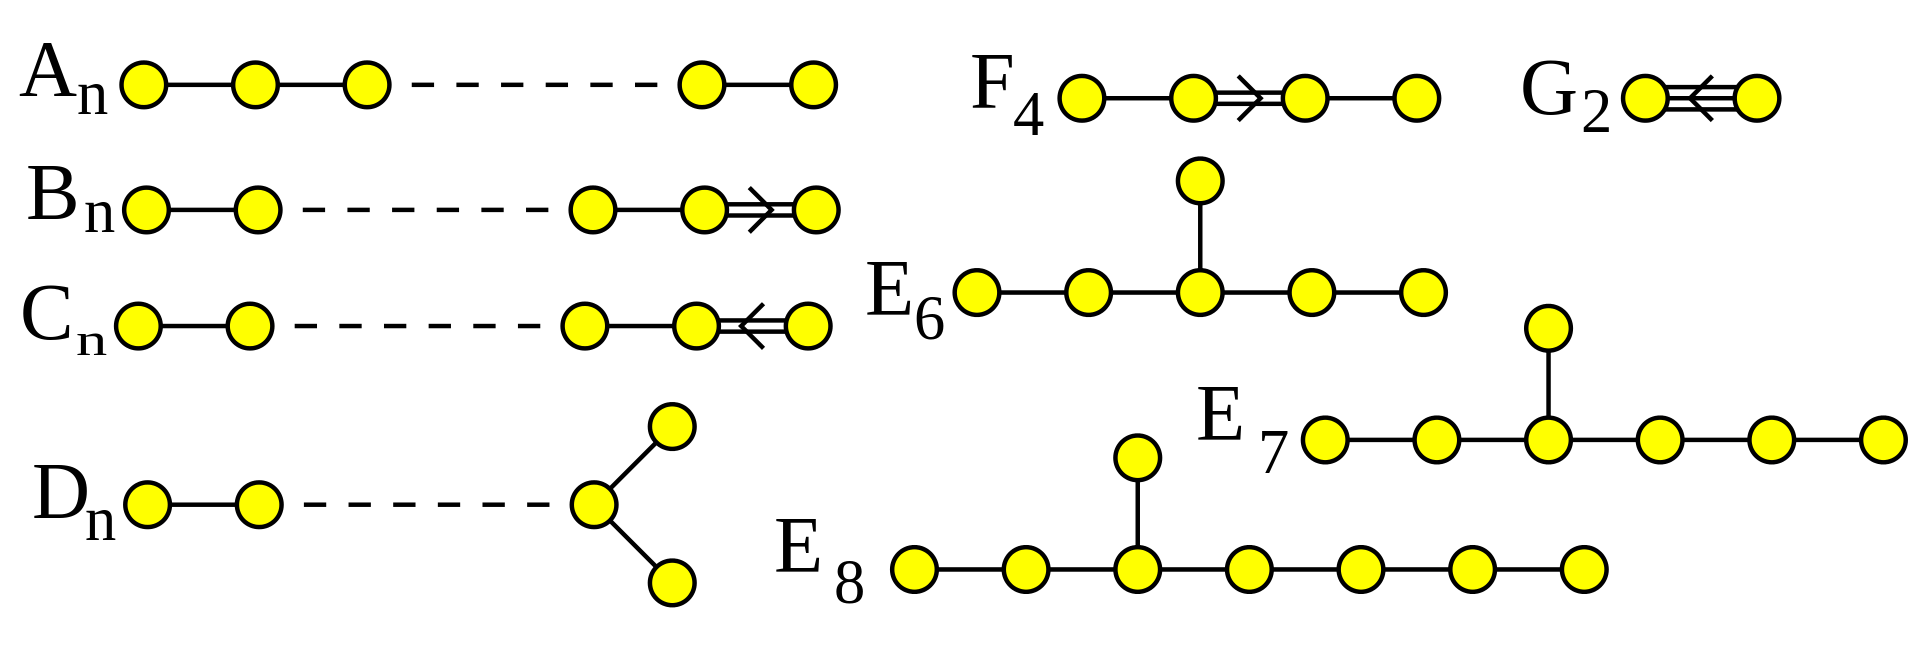
\includegraphics[width=0.5\linewidth]{finite_type_dynkin_diagrams.png}
                    \caption{Finite-type Dynkin diagrams}
                    \label{fig: finite_type_dynkin_diagrams}
                \end{figure}
                
                An easy consequence of the construction of Dynkin diagrams from finite-dimensional semi-simple Lie algebras (one checks whether or not the associated Cartan matrix decomposes into a block sum of two submatrices along the diagonal) is that the function:
                    $$\{ \text{Dynkin diagrams} \} \to \{ \text{finite-dimensional semi-simple Lie algebras over $k$} \}/\cong$$
                maps disjoint unions to direct sums and therefore, it suffices to ever only consider oneself with finite-dimensional simple Lie algebras. When a Dynkin diagram has only one connected component, we say that it is \textbf{connected}.
            \end{remark}
            The following result is a fundamental theorem in the study of finite-dimensional simple Lie algebras over algebraically closed fields of characteristic $0$. It essentially gives a bijective classification:
                $$\{ \text{connected Dynkin diagrams} \} \xrightarrow[]{\cong} \{ \text{finite-dimensional simple Lie algebras over $k$} \}/\cong$$
            which means that to give such a Lie algebra via a presentation by generators and relations is the same as giving its associated Cartan matrix. This is not only practically useful, but also is the mean by which one approaches Kac-Moody algebras, where the Cartan matrix is no longer required to be positive-definite (cf. \cite[Chapters 1-5]{kac_infinite_dimensional_lie_algebras}). 
            \begin{theorem}[Serre's Theorem]
                Let $\g$ be a finite-dimensional simple Lie algebra over an algebraically closed field of characteristic $0$ and denote its Cartan matrix by $(c_{ij})_{1 \leq i \leq l}$. Then, $\g$ is isomorphic to the Lie algebra generated by the set:
                    $$\{h_i, e_i^{\pm}\}_{1 \leq i \leq l}$$
                whose elements are subjected to the following relations, given for all $1 \leq i, j \leq l$:
                    $$[h_i, h_j] = 0$$
                    $$[h_i, e_j^{\pm}] = \pm c_{ij} e_j^{\pm}, [e_i^+, e_j^-] = \delta_{ij} h_i$$
                    $$\ad(e_i^{\pm})^{1 - c_{ij}}(e_j^{\pm}) = 0$$
                This is usually referred to as the \textbf{Chevalley-Serre} presentation for $\g$; final set of relations is usually known as the \textbf{Serre relations}.
            \end{theorem}
            \begin{corollary}
                For every root $\alpha \in \Phi$, any element $x \in \g[\alpha]$ is nilpotent under the vector representation of $\g$. 
            \end{corollary}
            \begin{corollary}[Triangular decomposition for finite-dimensional semi-simple Lie algebras]
                Let $\n^{\pm}$ denote the Lie subalgebras of $\g$ generated by the sets $\{e_i^{\pm}\}_{1 \leq i \leq l}$ respectively. Then:
                    $$\g \cong \n^- \oplus \h \oplus \n^+$$
                This is usually called the \textbf{triangular decomposition} for $\g$. 
            \end{corollary}

            We end this subsection with a brief analysis of the easiest possible example of a finite-dimensional simple Lie algebra. 
            \begin{example}[$\sl_2$]
                Recall that $\sl_2(k)$ is the kernel of the trace map:
                    $$\trace: \gl_2(k) \to k$$
                i.e. it is the Lie algebra of trace-zero $2 \x 2$-matrices whose Lie bracket is the usual commutator of matrices. It is of dimension $\dim_k \gl_2(k) - \dim_k k = 4 - 1 = 3$, and happens to be also generated by a set of cardinality $3$ (though this is a coincidence, due entirely to how \say{degenerate} of an example $\sl_2(k)$ is):
                    $$\{h, e^+, e^-\}$$
                and the elements of this set are subjected to the relations:
                    $$[h, e^{\pm}] = \pm 2 e^{\pm}, [e^+, e^-] = h$$
                One proves both of these statements by showing firstly that a basis for $\sl_2(k)$ is:
                    $$\left\{ \begin{pmatrix} 1 & 0 \\ 0 & -1 \end{pmatrix}, \begin{pmatrix} 0 & 1 \\ 0 & 0 \end{pmatrix}, \begin{pmatrix} 0 & 0 \\ 1 & 0 \end{pmatrix} \right\}$$
                and then seeing that any Cartan subalgebra of $\sl_2(k)$ must therefore be isomorphic to $k \begin{pmatrix} 1 & 0 \\ 0 & -1 \end{pmatrix}$; the rest then follows. In particular, the Cartan matrix is just:
                    $$\begin{pmatrix} 2 \end{pmatrix}$$
                and the Dynkin diagram consists of only a single vertex and no edges:
                    $$\bullet$$
                From this, one gathers that $\sl_2(k)$ is of type $\sfA_1$. 
            \end{example}

        \subsection{Perfect Lie algebras and their central extensions}
            \begin{definition}[Perfect Lie algebras]
                A Lie algebra over a commutative ring is said to be \textbf{perfect} if it is equal to its derived subalgebra. 
            \end{definition}
            \begin{example}
                Since semi-simple Lie algebras lack non-zero ideals by definition, they are perfect. 
            \end{example}

    \section{Kassel's realisation in terms of cyclic differential 1-forms}
        \begin{convention} \label{conv: a_fixed_finite_dimensional_simple_lie_algebra}
            From now on, we fix a finite-dimensional simple Lie algebra:
                $$\g$$
            over $\bbC$, equipped with a symmetric and non-degenerate invariant $\bbC$-bilinear form $(-, -)_{\g}$. It is known that such a bilinear form is unique up to $\bbC^{\x}$-multiples, so for all intents and purposes, it can be assumed to be the Killing form, though this assumption is not necessary. 
    
            Suppose also that $\g$ is equipped with a basis $\{x_i\}_{1 \leq i \leq \dim_{\bbC} \g}$ and with respect to $(-, -)_{\g}$, we identify a dual basis $\{x_i^*\}_{1 \leq i \leq \dim_{\bbC} \g}$. Recall that the Casimir tensor/canonical element of $\g$ is:
                $$\sfr_{\g} := \sum_{1 \leq i \leq \dim_{\bbC} \g} x_i \tensor x_i^* \in \g \tensor_{\bbC} \g^*$$
            and recall that $\sfr_{\g}$ is independent of what we choose the basis vectors $x_i$ to be.
    
            Eventually, we will also be concerned with the Dynkin diagram associated to the root system of $\g$. Let us denote this by:
                $$\Gamma := (\Gamma_0, \Gamma_1)$$
            wherein $\Gamma_0$ means the (finite) set of vertices and $\Gamma_1$ means the set of undirected edges between said vertices. 
    
            The set of all roots and respectively, positive/negative roots, and simple roots of $\g$ shall be denoted by:
                $$\Phi, \Phi^{\pm}, \Phi^{\circ}$$
            The set $\Phi^{\circ}$ is $\Z$-linearly independent and its $\Z$-span:
                $$Q := \Z \Phi^{\circ}$$
            is typically referred to as the root lattice of $\g$. Recall also that there is a set of fundamental weights: if we write:
                $$\check{\Phi}$$
            for the set of coroots of $\g$, then the so-called weight lattice of $\g$ shall be given by\footnote{We avoid the usual $\Delta$ notation, as we would like to reserve this symbol for a coproduct construction on affine Yangians.}:
                $$\Pi := \Hom_{\Z}(\check{Q}, \Z), \check{Q} := \Z\check{\Phi}$$
            inside which lies the set of fundamental weights, whose elements are dual to those of $\check{\Phi}^{\circ}$ (i.e. dual to simple coroots) with respect to $(-, -)_{\g}$\footnote{Which we might as well normalise so that $(\alpha_j, \check{\alpha}_j)_{\g} = 2$ for every $j \in \Gamma_0$, and hence the fundamental weights $\lambda_i$ will be simply be subjected to the relation $\delta_{ij} = 2 \frac{(\lambda_i, \check{\alpha}_i)_{\g}}{(\alpha_j, \check{\alpha}_j)_{\g}} = (\lambda_i, \check{\alpha}_i)_{\g}$.}.
        \end{convention}
    
        \subsection{A recollection of K\"ahler differentials}
            \begin{definition}[Modules of K\"ahler differentials] \label{def: kahler_differentials}
                
            \end{definition}
            The following well-known lemmas are very useful. A proof can be be found in any standard reference on general commutative algebra (cf. e.g. \cite[\href{https://stacks.math.columbia.edu/tag/00AO}{Tag 00AO}]{stacks}).
            \begin{lemma}[$1$-forms over polynomial algebras]
                \cite[\href{https://stacks.math.columbia.edu/tag/00RX}{Tag 00RX}]{stacks} Let $k$ be a commutative ring and fix some $n \in \Z_{\geq 0}$, and consider the canonical ring homomorphism $k \to k[v_1, ..., v_n]$. In this case, $\Omega^1_{[n]} := \Omega^1_{k[v_1, ..., v_n]/k}$ will be free and of finite rank $n$ as an $k[v_1, ..., v_n]$-module; in particular, it admits the set $\{dv_1, ..., dv_n\}$ as an $k[v_1, ..., v_n]$-linear basis. 
            \end{lemma}

        \subsection{Centres of UCEs of perfect Lie algebras}
            \begin{example}[Derived subalgebra of affine Kac-Moody algebras]
                
            \end{example}
    
    \addcontentsline{toc}{section}{References}
    \printbibliography

\end{document}